% SPDX-License-Identifier: AGPL-3.0-or-later
% Commercial license available
% © Concepts 1996-2026 Miroslav Sotek. All rights reserved.
% © Code 2020-2026 Miroslav Sotek. All rights reserved.
% ORCID: 0009-0009-3560-0851
% Contact: www.anulum.li | protoscience@anulum.li
% scpn-quantum-control --- S1 monitored-feedback control short paper

\documentclass[preprint,aps,physrev,superscriptaddress,floatfix,longbibliography]{revtex4-2}

\usepackage{amsmath,amssymb}
\usepackage{booktabs}
\usepackage{graphicx}
\usepackage{hyperref}
\usepackage{xcolor}
\usepackage{xurl}
\usepackage{siunitx}

\hypersetup{
    colorlinks=true,
    linkcolor=blue!60!black,
    citecolor=blue!60!black,
    urlcolor=blue!60!black,
}

\newcommand{\paperdoi}{Zenodo DOI: \href{https://doi.org/10.5281/zenodo.20382099}{10.5281/zenodo.20382099}}

\begin{document}
\emergencystretch=3em

\title{Monitored feedback versus open-loop control for Kuramoto--XY synchronisation on IBM dynamic circuits}

\author{Miroslav \v{S}otek}
\email{protoscience@anulum.li}
\affiliation{ANULUM, Marbach SG, Switzerland}
\affiliation{ORCID: 0009-0009-3560-0851}

\date{May 20, 2026\\\paperdoi}

\begin{abstract}
Dynamic circuits make it possible to test monitored quantum-control policies
on gate-model hardware rather than only static circuit families. We report a
preregistered four-qubit Kuramoto--XY feedback experiment on
\texttt{ibm\_kingston}. The payload uses three system qubits, one monitor
qubit, three dynamic rounds, and paired hardware arms: a monitored-feedback
arm and a matched open-loop control. The preregistered binary synchronisation
endpoint is negative: the feedback arm gives mean target error 0.2148958333,
while the matched control gives 0.2116406250, so the feedback policy does not
improve the selected target. We then replicate the full S1--S1f stack on
\texttt{ibm\_fez} and \texttt{ibm\_marrakesh}. The primary binary endpoint is
positive on those two backends, with target-error improvements 0.0927777778
and 0.0678710938, respectively. Direct-observable extensions show that this
is not a simple backend-independent controller promotion: Fez gives mostly
negative \texttt{YYI} extension structure, Marrakesh gives consistently
positive \texttt{YYI} and positive primary response, and the original
Kingston run remains a negative primary falsifier. The contribution is
therefore a hardware-control boundary result. A dedicated follow-up lane adds
full three-bit readout calibration and local gate-folding ZNE on Fez and
Marrakesh for S1b--S1f. Readout mitigation does not erase the
feedback/control separations, and ZNE generally preserves or enlarges them
except for the Fez S1f quadrature check. Paired dynamic-circuit feedback
tests and direct Pauli readouts can reveal backend- and calibration-window
sensitive response modes, but the tested controller is not supported as a
backend-general or robust synchronisation-improving policy. A same-layout
Marrakesh repeat remains positive, but with a smaller target-error
improvement, making drift robustness a measured constraint rather than an
assumption.
\end{abstract}

\maketitle

\section{Introduction}

Kuramoto synchronisation is a canonical model for collective phase dynamics
and has a long history in nonlinear science~\cite{Kuramoto1975,Acebron2005}.
Gate-model quantum circuits can encode small XY-type phase-coupled systems,
but noisy intermediate-scale quantum hardware requires conservative claim
boundaries~\cite{Preskill2018,NielsenChuang2010}. In this setting, the
scientific question is not whether a broad quantum advantage has been shown.
The useful question is narrower: can a small monitored feedback policy improve
a preregistered hardware observable relative to a matched open-loop arm under
the same backend, layout, shot budget, repetitions, and calibration window?

This work is the dynamic-circuit control branch of the same Kuramoto--XY
hardware programme that produced the DLA-parity leakage observation, the FIM
hardware falsification, and the reduced-Pauli mechanism-separation
study~\cite{SotekDLA2026,SotekFIM2026,SotekPhase3ReducedPauli2026}. Its role is
not to promote a controller after one positive backend response. It asks
whether monitored feedback has a reproducible paired-arm signature once direct
observables, backend replication, readout calibration, and local-folding ZNE
are all treated as part of the claim boundary.

Measurement-conditioned feedback is a standard quantum-control primitive
~\cite{WisemanMilburn2010}. Dynamic circuits provide the required gate-model
hardware surface: mid-circuit measurement, classical conditioning, and
subsequent gates within one submitted payload
~\cite{Corcoles2021,IBMQuantum,Qiskit2024}. Mid-circuit readout has also
become a practical resource for near-term quantum simulation
~\cite{Koh2023}, and adaptive circuits can express tasks unavailable to
fixed-depth unitary circuits at the same depth~\cite{FossFeig2023}. They also
create a stricter experimental standard. A feedback arm alone is not
interpretable, because backend drift, layout selection, readout bias, and
ordinary shot noise can all masquerade as control response. The S1 experiment
therefore uses a paired-arm design: every feedback run is compared with a
matched open-loop control generated from the same circuit body and executed in
the same hardware window.

This paper reports the completed S1 hardware programme. The primary
preregistered binary proxy is negative. The same-paper extensions then ask
whether the negative proxy hides smaller channel-level responses in direct
XY-sector observables. The final result is scientifically useful, but
conservative: the tested controller is not promoted. Instead, the paired-arm
method identifies a structured failure and sensitivity boundary for future
redesigned feedback policies.

\section{Preregistered S1 protocol}

The primary S1 payload uses three system qubits and one monitor qubit. The
feedback arm runs three dynamic rounds. In each round, the monitor qubit is
coupled to the system, measured, unconditionally reset, and used to condition a
small correction on the system. The matched open-loop arm preserves the same
body structure without using the measured monitor outcome as an active
feedback signal. The readiness artefact is generated by the committed S1
readiness script, and the canonical preregistration package is the JSON file
dated May 6, 2026 under \path{data/s1_feedback_loop/}.
The live payload used unconditional monitor reset and conditional correction
only, because the submitted provider path rejected reset operations inside
conditional blocks. This implementation detail is part of the experimental
boundary: the circuit tests provider-supported dynamic-circuit feedback, not
arbitrary low-latency real-time control.

\begin{table}[tb]
\centering
\begin{tabular}{lr}
\toprule
Protocol field & Value \\
\midrule
System qubits & 3 \\
Monitor qubits & 1 \\
Classical bits & 6 \\
Dynamic rounds & 3 \\
Hardware arms & feedback, matched open-loop control \\
Primary circuits & 2 \\
Shots per circuit & 1024 \\
Repetitions per arm & 12 \\
Target synchronisation proxy & 0.72 \\
\bottomrule
\end{tabular}
\caption{Primary S1 preregistered dynamic-circuit payload.}
\label{tab:protocol}
\end{table}

The primary endpoint is the absolute target-order-parameter error,
\begin{equation}
    \epsilon_{\mathrm{target}} = |R_{\mathrm{live}} - R_{\mathrm{target}}|,
\end{equation}
where $R_{\mathrm{target}}=0.72$. The feedback arm is useful under the
preregistered decision rule only if it reduces this error relative to the
matched open-loop control.

\section{Direct-observable extensions}

The primary binary proxy saturates near one on the selected backend. To avoid
over-interpreting a single nearly saturated readout, S1 includes a series of
same-paper direct-observable extensions. These are not separate papers and do
not change the primary endpoint. They localise the failure mode by measuring
XY-sector and control observables from matched feedback/control arms.

S1b preserves the original dynamic feedback body and measures final
\texttt{IXX}, \texttt{IYY}, \texttt{XXI}, and \texttt{YYI} correlators.
S1c reduces the body to one dynamic round, correction angle 0.06, and base
gain 0.4. S1d compares three preregistered one-round policy variants:
\texttt{current\_shallow\_positive}, \texttt{polarity\_flipped}, and
\texttt{weak\_positive}. S1e repeats that policy sweep at five repetitions per
arm. S1f keeps the S1d/S1e-favoured shallow policy and measures \texttt{XXI},
\texttt{XYI}, \texttt{YXI}, \texttt{YYI}, and \texttt{ZZI}. The
\texttt{XYI}/\texttt{YXI} rows test cross-quadrature leakage, while
\texttt{ZZI} is a population-sector control.

Figure~\ref{fig:s1-heatmap} gives the extension-level summary across
\texttt{ibm\_kingston}, \texttt{ibm\_fez}, and \texttt{ibm\_marrakesh}. The
figure is intended to expose the same logic as the tables: the direct
observable response is structured, but its sign and localisation are
backend-dependent.

For an observable $P$, each arm expectation is reduced from counts as
\begin{equation}
    \langle P \rangle =
    \frac{1}{N}\sum_b n_b \prod_{i\in \mathrm{supp}(P)}(-1)^{b_i},
\end{equation}

\begin{figure}[tb]
\centering
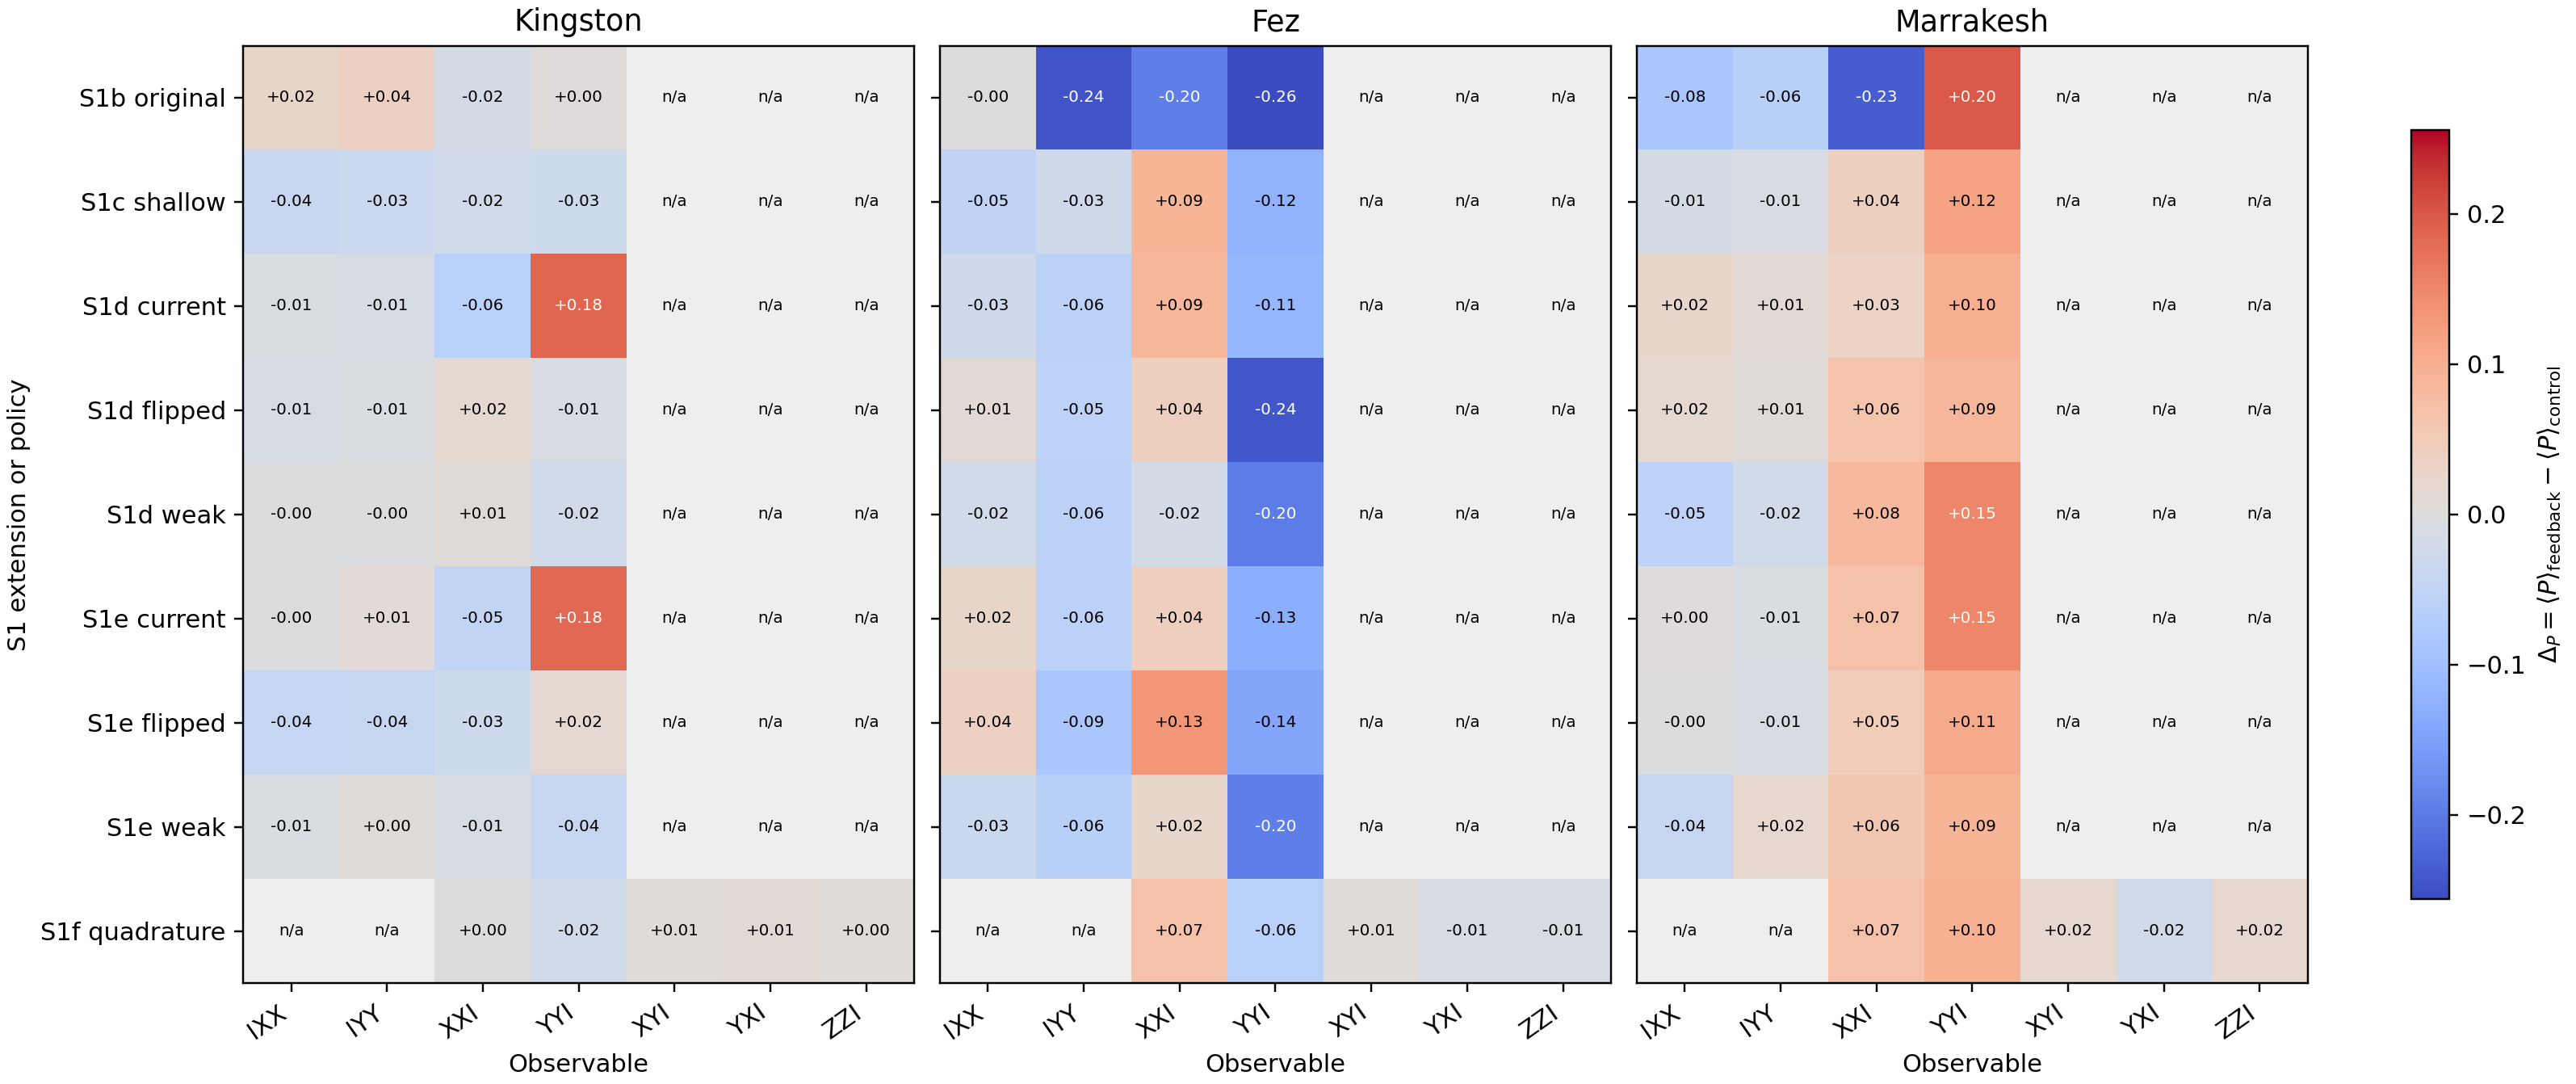
\includegraphics[width=0.98\linewidth]{figures/s1_feedback_control/s1_feedback_multibackend_delta_heatmap_2026-05-20.png}
\caption{Feedback-minus-control Pauli expectations across the S1 direct
observable extensions on three IBM Heron backends. Grey cells mark
observables not included in that extension. The original Kingston
\texttt{YYI} feature is not backend-universal: Fez is mostly negative in the
\texttt{YYI} column, while Marrakesh is positive through the shallow policy
and quadrature checks.}
\label{fig:s1-heatmap}
\end{figure}
with $n_b$ the observed count for bitstring $b$ and $N$ the total shots. The
reported extension quantity is
\begin{equation}
    \Delta_P =
    \langle P\rangle_{\mathrm{feedback}} -
    \langle P\rangle_{\mathrm{control}}.
\end{equation}

\section{Primary S1 result and replication}

The primary paired-arm execution first completed on \texttt{ibm\_kingston}.
The feedback job was \texttt{d86qn3lg7okc73elg2eg}; the matched open-loop
control job was \texttt{d86qn65g7okc73elg2hg}. Each arm used 12 repetitions
and 12,288 total shots. The transpiled depths were 717 for the feedback arm
and 684 for the matched control. This first execution was negative under the
preregistered decision tree.

After review, the same primary endpoint was replicated on \texttt{ibm\_fez}
and \texttt{ibm\_marrakesh}. The Fez jobs were
\texttt{d86sl45g7okc73elimdg} and \texttt{d86slcp789is73904bng}. The
Marrakesh jobs were \texttt{d86sr9h789is73904jm0} and
\texttt{d86src2s46sc73f7edm0}. Both same-day replication runs were positive
on the binary target-error endpoint, as shown in Table~\ref{tab:s1-primary}.
A later Marrakesh same-layout repeat pinned to system qubits [7,17,6] and
monitor qubit 8 also remained positive. Its jobs were
\texttt{d86tk8op0eas73dlf4pg} and \texttt{d86tkbp789is73905hkg}. The repeat
reduced the effect size from 0.0678710938 to 0.0036935764, so it supports the
sign of the Marrakesh primary response but not calibration-window invariance.

\begin{table}[tb]
\centering
\small
\begin{tabular}{lrrrr}
\toprule
Backend & Feedback error & Control error & Improvement & Decision \\
\midrule
\texttt{ibm\_kingston} & 0.2148958333 & 0.2116406250 & -0.0032552083 & negative \\
\texttt{ibm\_fez} & 0.0355338542 & 0.1283116319 & 0.0927777778 & positive \\
\texttt{ibm\_marrakesh} & 0.0440559896 & 0.1119270833 & 0.0678710938 & positive \\
\texttt{ibm\_marrakesh} repeat & 0.0232183160 & 0.0269118924 & 0.0036935764 & positive \\
\bottomrule
\end{tabular}
\caption{Primary S1 binary-proxy hardware result across three backends. The
improvement column is control target error minus feedback target error, so
positive values favour feedback. The final row is a same-layout Marrakesh
repeat on physical layout [7,17,6,8].}
\label{tab:s1-primary}
\end{table}

The primary result is therefore not a universal controller failure, but it is
also not a backend-general controller success. The same preregistered
three-round payload is negative on Kingston and positive on Fez and
Marrakesh. This makes backend and calibration-window dependence part of the
main result rather than a footnote. The direct-observable stack below is
needed to determine whether the positive primary endpoint corresponds to a
stable mechanism.

\section{XY-sector localisation}

S1b asks whether the negative binary endpoint hides channel-level differences
in direct XY-sector observables. The original dynamic feedback body is
preserved, but the final basis is rotated to the selected Pauli correlator.
The results are shown in Table~\ref{tab:s1bc}.

\begin{table}[tb]
\centering
\begin{tabular}{lrr}
\toprule
Observable & S1b $\Delta_P$ & S1c $\Delta_P$ \\
\midrule
\texttt{IXX} & 0.0247395833 & -0.0364583333 \\
\texttt{IYY} & 0.0358072917 & -0.0319010417 \\
\texttt{XXI} & -0.0175781250 & -0.0221354167 \\
\texttt{YYI} & 0.0039062500 & -0.0292968750 \\
\midrule
Mean $|\Delta_P|$ & 0.0205078125 & 0.0299479167 \\
\bottomrule
\end{tabular}
\caption{S1b direct XY-sector extension and S1c shallow/gain-tuned extension.
S1b is mixed-sign; S1c is negative in all four channels.}
\label{tab:s1bc}
\end{table}

S1b is not a positive controller result. Three channels move in the feedback
direction and one moves against it, with mean absolute separation only
0.0205078125. It is, however, more informative than the saturated binary
proxy: the feedback/control difference is channel-structured rather than
uniformly absent.

S1c then tests whether the depth and gain of the original dynamic body are the
problem. The shallower, lower-gain policy reduces the feedback depths to about
237, but all four XY-sector channels move negative. The direct-observable
response therefore cannot be rescued by this shallow/gain-tuned policy on
Kingston. The Fez and Marrakesh replications show a different boundary: the
same direct-observable lanes have larger aggregate separations than Kingston,
but their channel signs disagree. Fez is dominated by negative
\texttt{YYI}/\texttt{IYY} structure, whereas Marrakesh has a persistent
positive \texttt{YYI} column.

\section{Policy-direction sweep and repeat}

S1d compares three one-round policy variants. S1e repeats the same policy
sweep at five repetitions per arm. The purpose is to distinguish a genuine
policy-direction response from a single noisy calibration window. The results
are shown in Table~\ref{tab:s1de}. The artefact timestamps place S1d at
13:46:14Z and S1e at 14:09:19Z on May 20, 2026, a separation of about
23 minutes under the same backend family and day.

\begin{table*}[tb]
\centering
\scriptsize
\begin{tabular}{@{}llrrrrrr@{}}
\toprule
Run & Variant & \texttt{IXX} & \texttt{IYY} & \texttt{XXI} & \texttt{YYI} & Mean signed & Mean abs. \\
\midrule
S1d & \texttt{current\_shallow\_positive} & -0.007813 & -0.013672 & -0.060547 & 0.184896 & 0.025716 & 0.066732 \\
S1d & \texttt{polarity\_flipped} & -0.013021 & -0.006510 & 0.015625 & -0.012370 & -0.004069 & 0.011882 \\
S1d & \texttt{weak\_positive} & -0.002604 & -0.003906 & 0.006510 & -0.020182 & -0.005046 & 0.008301 \\
\midrule
S1e & \texttt{current\_shallow\_positive} & -0.003516 & 0.008203 & -0.048828 & 0.182422 & 0.034570 & 0.060742 \\
S1e & \texttt{polarity\_flipped} & -0.042969 & -0.040625 & -0.028125 & 0.016797 & -0.023730 & 0.032129 \\
S1e & \texttt{weak\_positive} & -0.007422 & 0.004297 & -0.010547 & -0.040625 & -0.013574 & 0.015723 \\
\bottomrule
\end{tabular}
\caption{S1d policy-direction sweep and S1e higher-repetition repeat. Values
are feedback-minus-control Pauli expectations.}
\label{tab:s1de}
\end{table*}

The same narrow feature appears in both S1d and S1e:
\texttt{current\_shallow\_positive} has a large positive \texttt{YYI}
separation, 0.1848958333 in S1d and 0.1824218750 in S1e. The alternative
policies remain close to zero or negative by mean signed separation. This is a
real policy-sensitive signal candidate, but it is too narrow for controller
promotion: \texttt{IXX} and \texttt{XXI} remain negative for the same policy,
and the favourable aggregate is driven by one channel.

\section{Quadrature mechanism check}

S1f is the final same-paper discriminator. It keeps
\texttt{current\_shallow\_positive} and tests whether the repeated
\texttt{YYI} response belongs to a stable quadrature structure. It measures
the original \texttt{XXI}/\texttt{YYI} pair, the cross-quadrature controls
\texttt{XYI}/\texttt{YXI}, and a population control \texttt{ZZI}. The result
is shown in Table~\ref{tab:s1f}. Its artefact timestamp is 14:22:13Z, about
13 minutes after S1e and about 103 minutes after the primary S1 paired-arm
timestamp. This is therefore a later same-day calibration-window check, not a
multi-day stability claim.

\begin{table}[tb]
\centering
\begin{tabular}{lrrr}
\toprule
Observable & Feedback & Control & $\Delta_P$ \\
\midrule
\texttt{XXI} & 0.2187500000 & 0.2175781250 & 0.0011718750 \\
\texttt{XYI} & 0.1617187500 & 0.1566406250 & 0.0050781250 \\
\texttt{YXI} & 0.2242187500 & 0.2136718750 & 0.0105468750 \\
\texttt{YYI} & -0.0445312500 & -0.0242187500 & -0.0203125000 \\
\texttt{ZZI} & 0.6523437500 & 0.6480468750 & 0.0042968750 \\
\midrule
Mean $|\Delta_P|$ & \multicolumn{2}{r}{ } & 0.0082812500 \\
\bottomrule
\end{tabular}
\caption{S1f quadrature and population-control check. The large positive
\texttt{YYI} response seen in S1d/S1e does not persist in this later window.}
\label{tab:s1f}
\end{table}

The S1f result blocks the strongest possible positive interpretation of S1d
and S1e on Kingston. The \texttt{YYI} separation changes sign and the mean
absolute feedback--control separation falls to 0.0082812500. The
cross-quadrature controls are small, and the population control is also small.
On Fez, S1f remains negative in \texttt{YYI} with mean absolute separation
0.0314843750. On Marrakesh, S1f remains positive in \texttt{YYI} with mean
absolute separation 0.0453125000. The conservative interpretation is not a
stable backend-general quadrature-localised feedback mechanism; it is a
backend-dependent response boundary.

\begin{table*}[tb]
\centering
\scriptsize
\resizebox{\textwidth}{!}{%
\begin{tabular}{lrrrrrrr}
\toprule
Backend & Primary improvement & S1b mean abs. & S1c mean abs. &
S1d current \texttt{YYI} & S1e current \texttt{YYI} &
S1f \texttt{YYI} & S1f mean abs. \\
\midrule
\texttt{ibm\_kingston} & -0.003255 & 0.020508 & 0.029948 & 0.184896 & 0.182422 & -0.020313 & 0.008281 \\
\texttt{ibm\_fez} & 0.092778 & 0.173991 & 0.071777 & -0.114583 & -0.128906 & -0.060547 & 0.031484 \\
\texttt{ibm\_marrakesh} & 0.067871 & 0.145182 & 0.044596 & 0.099609 & 0.148047 & 0.096875 & 0.045313 \\
\bottomrule
\end{tabular}
}
\caption{Compact cross-backend S1--S1f summary. The primary improvement is
control target error minus feedback target error. Direct-observable entries
are feedback-minus-control Pauli expectations or mean absolute separations.}
\label{tab:cross-backend-summary}
\end{table*}

\section{Readout mitigation and ZNE stress lane}

The first S1b--S1f direct-observable executions did not include dedicated
readout calibration circuits. We therefore do not retrofit mitigation onto
those artefacts. Instead, we execute a new preregistered readout/ZNE lane on
Fez and Marrakesh. Each backend/lane submission contains the folded main
circuits at local gate-folding noise scales 1, 3, and 5, plus all eight
computational-basis calibration circuits for the three final system-readout
bits. The calibration and main circuits are pinned to the same selected
system/monitor physical layout. The folding is local rather than global
unitary folding because the S1 feedback arm contains mid-circuit measurement,
reset, and classical conditioning; the reducer folds invertible quantum gates
while preserving the dynamic-circuit control-flow operations.

\begin{table*}[tb]
\centering
\scriptsize
\resizebox{\textwidth}{!}{%
\begin{tabular}{llrrrr}
\toprule
Backend & Lane & Scale-1 mean abs. & Linear ZNE mean abs. &
Readout-mitigated linear ZNE mean abs. & Readout matrix cond. \\
\midrule
\texttt{ibm\_fez} & S1b & 0.056315 & 0.063192 & 0.063868 & 1.078215 \\
\texttt{ibm\_fez} & S1c & 0.031738 & 0.038425 & 0.039430 & 1.059059 \\
\texttt{ibm\_fez} & S1d & 0.038032 & 0.043936 & 0.045297 & 1.059970 \\
\texttt{ibm\_fez} & S1e & 0.037435 & 0.045204 & 0.046707 & 1.061207 \\
\texttt{ibm\_fez} & S1f & 0.054141 & 0.041439 & 0.042975 & 1.066406 \\
\midrule
\texttt{ibm\_marrakesh} & S1b & 0.030273 & 0.040256 & 0.040437 & 1.036386 \\
\texttt{ibm\_marrakesh} & S1c & 0.113932 & 0.120402 & 0.122239 & 1.029654 \\
\texttt{ibm\_marrakesh} & S1d & 0.095486 & 0.101951 & 0.102965 & 1.031348 \\
\texttt{ibm\_marrakesh} & S1e & 0.104590 & 0.113810 & 0.115997 & 1.038547 \\
\texttt{ibm\_marrakesh} & S1f & 0.069531 & 0.076432 & 0.077617 & 1.040666 \\
\bottomrule
\end{tabular}
}
\caption{Dedicated readout-mitigation and local-folding ZNE lane for the S1
direct-observable stack. The table reports mean absolute
feedback-minus-control separation across each lane's preregistered Pauli
channels or policy-channel rows. The readout confusion matrices are
well-conditioned in this lane; mitigation does not remove the observed
separations.}
\label{tab:s1-readout-zne}
\end{table*}

Table~\ref{tab:s1-readout-zne} changes the limitation boundary. The dominant
direct-observable separations are not explained away by a poorly conditioned
readout inversion: the full-basis readout matrices have condition numbers
near one, and the readout-mitigated ZNE values remain close to the unmitigated
ZNE values. The ZNE stress test also does not convert the result into a
controller-promotion claim. On Marrakesh, all S1b--S1f mean absolute
separations increase under the linear ZNE fit. On Fez, S1b--S1e also increase,
while S1f decreases. The conservative interpretation is that the
feedback/control response is not a simple removable readout artefact, but the
sign and localisation remain backend- and lane-dependent.

\section{Provider constraints and controller redesign}

The revised S1 analysis records provider constraints as experimental
variables. Both Fez and Marrakesh reported \SI{4}{\nano\second} values for
\texttt{dt} and \texttt{dtm} in the runtime backend snapshot. The target
timing constraints exposed by the Qiskit target were acquire alignment 1,
pulse alignment 1, granularity 1, and minimum pulse length 2. The provider API
used for this manuscript did not expose a per-branch classical-conditioning
latency or reset fidelity value. We therefore do not quote a fabricated
latency or reset number. Instead, the measured dynamic-circuit cost boundary
is the transpiled control-flow structure: on the same-layout Marrakesh repeat,
the feedback arm has maximum transpiled depth 715 with three
\texttt{if\_else} operations, six measurements, and three resets; the matched
control has maximum transpiled depth 696 with six measurements and three
resets. On the Fez primary replication, the corresponding depths are 717 and
684.

\begin{table}[tb]
\centering
\scriptsize
\begin{tabular}{lrrrr}
\toprule
Backend & Mean readout error & Mean retention & Max leakage & Multi-bit proxy \\
\midrule
\texttt{ibm\_fez} & 0.010895 & 0.974121 & 0.040430 & 0.000293 \\
\texttt{ibm\_marrakesh} & 0.006378 & 0.985718 & 0.023242 & 0.000073 \\
\bottomrule
\end{tabular}
\caption{Provider and calibration constraints for the S1 readout/ZNE layouts.
The mean readout error is taken from the live backend properties on the
selected four-qubit layout. Mean retention, max leakage, and multi-bit proxy
come from the dedicated final-readout calibration circuits, averaged across
S1b--S1f. The multi-bit proxy is the observed probability of a calibration
outcome differing from the prepared state in at least two final-readout bits;
it is not mid-circuit crosstalk tomography.}
\label{tab:provider-constraints}
\end{table}

These constraints motivate a concrete next controller rather than a generic
``try again'' loop. The next S1 controller should replace the fixed correction
angle with a monitor-conditioned signed gain: the correction amplitude should
depend on the monitor outcome and on a preregistered confidence map derived
from the calibration lane. It should add a two-monitor variant that separately
observes the edge associated with the \texttt{YYI} response and an orthogonal
control edge, so that a single monitor cannot ambiguously couple policy signal
and readout pathway. Finally, it should test an explicit topology variant
that targets the \texttt{YYI}-sensitive edge seen on Marrakesh while carrying
the same polarity, cross-quadrature, and population controls used here. The
acceptance gate for such a controller should require the primary binary proxy,
the preregistered \texttt{YYI} direct observable, and a same-layout repeat to
agree in sign before any controller-promotion claim is made.

\section{Reproducibility artefacts}

The hardware evidence is committed as raw-count and analysis artefacts under
\path{data/s1_feedback_loop/}. Table~\ref{tab:artefacts} lists the primary
analysis artefacts and SHA256 digests used for this manuscript. The exact
hardware job identifiers are retained in the JSON files and in the Markdown
draft notes.

\begin{table*}[tb]
\centering
\small
\begin{tabular}{p{0.08\textwidth}p{0.34\textwidth}p{0.46\textwidth}}
\toprule
Run & Analysis artefact & SHA256 \\
\midrule
S1 & \path{s1_feedback_analysis_summary_ibm_kingston_20260520T123941Z.json} & \path{dcfae0016806ac3f705ce9ecad62f1ab47d0d3986775170a7f15b380f38fcf24} \\
S1b & \path{s1b_xy_observable_analysis_ibm_kingston_20260520T130238Z.json} & \path{91fdedc8043d25c68f95a57c21be7ed828c7e83f34af48f11010fae686e4b152} \\
S1c & \path{s1c_xy_observable_analysis_ibm_kingston_20260520T132455Z.json} & \path{ade9a407dec9759ed4fe789f738d4ff3560f2ecf73561f6f07435c4bab9f50dd} \\
S1d & \path{s1d_xy_observable_analysis_ibm_kingston_20260520T134614Z.json} & \path{6e6bc2f513f23633c72756016392b58cbf140d89c6f9cc7fdd07880c66b61c76} \\
S1e & \path{s1e_xy_observable_analysis_ibm_kingston_20260520T140919Z.json} & \path{4f7e106e2af8e42aa74c9c07d66032bc76a78a936c499370c56fcef8c32ad522} \\
S1f & \path{s1f_xy_observable_analysis_ibm_kingston_20260520T142213Z.json} & \path{17b37753460137c796a5fb8c52784ce694d7ce4ffb63e55c92853abe8f91313e} \\
\bottomrule
\end{tabular}
\caption{Committed analysis artefacts supporting the S1--S1f manuscript.}
\label{tab:artefacts}
\end{table*}

The Fez and Marrakesh replication artefacts follow the same naming scheme
under \path{data/s1_feedback_loop/}, with backend names
\texttt{ibm\_fez} and \texttt{ibm\_marrakesh} and timestamps
20260520T145159Z--20260520T150249Z for Fez and
20260520T150509Z--20260520T151450Z for Marrakesh. Their analysis SHA256
digests are recorded in the JSON sidecars and in the repository history.
The dedicated readout/ZNE lane uses timestamps 20260520T153231Z--20260520T153820Z
for Fez and 20260520T153231Z--20260520T153847Z for Marrakesh. Its job IDs are
\texttt{d86t84p789is739052r0}, \texttt{d86t8ftg7okc73eljf10},
\texttt{d86t8qp789is739053og}, \texttt{d86t9hop0eas73dleo20}, and
\texttt{d86tarlg7okc73elji20} on Fez, and
\texttt{d86t84op0eas73dlem4g}, \texttt{d86t8gtg7okc73eljf20},
\texttt{d86t8stg7okc73eljfig}, \texttt{d86t9ptg7okc73eljgo0}, and
\texttt{d86tb2dg7okc73eljiag} on Marrakesh. The same-layout Marrakesh repeat
analysis artefact is
\path{s1_feedback_analysis_summary_ibm_marrakesh_20260520T155826Z.json};
the provider-constraint artefact is
\path{s1_dynamic_circuit_constraints_20260520T160234Z.json}.

\section{Claim boundary}

The supported claims are deliberately narrow. First, the S1 monitored-feedback
payload and matched open-loop control executed on three IBM Heron backends,
with a negative primary result on Kingston and positive primary results on
Fez and Marrakesh. Second, direct XY-sector extensions show that
feedback/control differences can be channel-structured and policy-sensitive.
Third, the S1d/S1e/S1f \texttt{YYI} story is backend-dependent: Kingston loses
the positive \texttt{YYI} response in S1f, Fez is mostly negative in that
column, and Marrakesh remains positive. The controller is therefore not
promoted as backend-general.

The paper does not claim quantum advantage, backend-general feedback control,
full real-time control beyond provider-supported dynamic circuits, scalable
control, or larger-system synchronisation. It also does not claim that the
observed response is isolated from calibration drift, layout-dependent
coherent error, readout effects, or finite-shot variation. The result is a
bounded hardware-control measurement and a falsifier for the tested feedback
law as a universal policy.

At the time of execution, authenticated live QPU access for this campaign was
limited to IBM Quantum hardware and to the three Heron backends reported here.
The framework contains provider-neutral execution and packaging surfaces for
other gate-model, trapped-ion, neutral-atom, photonic, annealing, analogue, and
simulator targets, but those software routes are not evidence of live
non-IBM execution. We plan to rerun the same preregistered S1 payloads on
additional hardware families when compute allocations and provider access
become available; until those reruns exist, no cross-provider or
cross-technology controller claim is made.

The original S1b--S1f artefacts remain unmitigated raw hardware evidence. The
readout/ZNE lane is a separate preregistered execution, not a post hoc
correction of those earlier jobs. Mid-circuit measurement and feedforward
readout mitigation is an active technical area~\cite{KohKohThompson2026};
the present reducer only mitigates the final three-bit readout distribution
and only stress-tests gate noise through local folding of invertible quantum
operations.

\section{Discussion}

The central scientific value of S1 is methodological rather than promotional.
The primary endpoint fails on Kingston but succeeds on Fez and Marrakesh, so a
single-backend story would be misleading in either direction. The extensions
then add mechanism information that a binary endpoint alone would hide. S1b
and S1c show backend-dependent XY-sector response; S1d and S1e show that the
policy sweep can repeat a \texttt{YYI} feature inside a backend window; and
S1f shows that the same feature is not stable across backends. The dedicated
readout/ZNE lane strengthens the negative claim boundary: the
direct-observable separations survive full final-readout calibration and do
not behave like a uniform monotone gate-noise artefact.

This sequence is useful for future control design because it converts a
simple negative result into design constraints. Any next-generation S1 policy
must preregister direct Pauli observables rather than rely only on the binary
proxy. It must include a matched open-loop arm, policy-polarity controls,
cross-quadrature controls, and a population control. It should also reserve a
same-layout repeat in a later calibration window before promoting a
controller. It should additionally treat provider constraints as first-class
experimental variables: mid-circuit measurements and resets add latency,
classical conditioning changes the transpiled control-flow path, reset
fidelity can couple the monitor qubit back into subsequent rounds, and
measurement crosstalk can affect both the monitored branch and the final
readout. Deterministic error-suppression and calibration-aware workflows can
improve near-term algorithm performance~\cite{Mundada2023}, but S1 shows that
the feedback law itself still needs a matched-arm falsification gate. Under
these standards, S1 is not archive clutter: it is a claim-bound falsification
and localisation paper for dynamic-circuit feedback on current IBM hardware.

\begin{figure}[tb]
\centering
\fbox{\begin{minipage}{0.92\linewidth}
\small
\begin{tabular}{@{}p{0.25\linewidth}p{0.66\linewidth}@{}}
Monitor layer & Mid-circuit measurement with reset-fidelity and latency
metadata recorded before execution. \\
Adaptive policy & Outcome-conditioned gain and polarity selected from a
preregistered finite policy table. \\
Control arm & Matched open-loop body with the same routed circuit family and
shot budget. \\
Observable gate & Binary proxy plus direct \texttt{XX}/\texttt{YY},
cross-quadrature, and population controls. \\
Promotion gate & Same-layout repeat and readout/ZNE lane before any
backend-specific controller promotion. \\
\end{tabular}
\end{minipage}}
\caption{Concrete redesign target implied by S1. The next controller should
make provider constraints and direct observables part of the preregistered
policy, rather than treating them as post-run diagnostics.}
\label{fig:controller-redesign}
\end{figure}

\section{Conclusion}

The S1 programme tests monitored feedback at the smallest scale where IBM
dynamic circuits can implement an active monitor-and-correct loop with a
matched open-loop control. The preregistered binary synchronisation endpoint
is negative on Kingston but positive on Fez and Marrakesh. Direct-observable
extensions reveal structured, policy-sensitive feedback/control differences,
and a dedicated Fez/Marrakesh readout/ZNE lane shows that those differences
are not erased by full final-readout mitigation or by local-folding
extrapolation. The final quadrature checks still do not support a
backend-general positive controller mechanism. The appropriate publication
claim is therefore precise: S1 establishes a reproducible paired-arm method
and a hardware-control boundary for Kuramoto--XY feedback, while rejecting
backend-general promotion of the tested controller. It also establishes that
monitored feedback on IBM dynamic circuits can exhibit backend-dependent
response modes that are not captured by a saturated binary synchronisation
proxy, which is a concrete methodological constraint for future controller
design.

\bibliographystyle{apsrev4-2}
\bibliography{s1_feedback_control_refs}

\end{document}
